\section{\freest{} is for programming}
\label{sec:programming}

\freest{} is a basic implementation of the language introduced by
Thiemann and Vasconcelos~\cite{DBLP:conf/icfp/ThiemannV16}. Here we
provide a gentle introduction to the language.
%
We have chosen the concrete syntax to be aligned with that of Haskell,
as much as possible. A \freest{} script is a collection of type
abbreviations, datatype and function (or value) declarations. Function
\lstinline|start| starts it all.

Our first example serializes a tree object on a channel. The datatype
for trees, \lstinline|Tree|, was introduced before.  We also need a
channel capable of transmitting a tree. The type below describes a
variant of the \lstinline|TreeChannel| introduced before that not only
sends a tree, but, for each \lstinline|Node|, also receives back an
integer value.
%
\begin{lstlisting}
type TreeC = +{Leaf: Skip, Node: !Int;TreeC;TreeC;?Int}
\end{lstlisting}

The \lstinline|+| type constructor introduces an internal choice (the
process in possession of the channel end chooses) with two
alternatives, labelled \lstinline|Leaf| and \lstinline|Node|. These
two labels should not be confused with the constructors of 
datatype \lstinline|Tree|. \lstinline|Leaf| states that no further
interaction is possible on the channel (denoted by \lstinline|Skip|);
the \lstinline|Node| branch writes an integer value, followed by two
trees, and terminates by reading an integer value
(\lstinline|!Int;TreeC;TreeC;?Int|).
%
The type declaration introduces an \emph{abbreviation} to a recursive
type \lstinline|rec x. +{Leaf: Skip, Node: !Int;x;x;?Int}|, a type
that is valid in \freest.

The writer process, \lstinline|transform|, writes a tree on a given
channel. The channel is of type \lstinline|TreeC;alpha|, for
a type variable \lstinline|alpha|. It returns a \lstinline|Tree| and
the residual of the input channel, of type \lstinline|alpha|. The type
of \lstinline|transform| is \emph{polymorphic}: different calls to the
function use different values for \lstinline|alpha|.

\begin{lstlisting}
transform: forall alpha => Tree -> TreeC;alpha -> (Tree, alpha)
\end{lstlisting}

For each \lstinline|Node| in the input tree, function
\lstinline|transform| reads an integer from the channel and returns a
tree isomorphic to the input where the integer values in nodes are
read from the channel.
%
The function performs a \lstinline|case| analysis on the
\lstinline|Tree| constructor (either \lstinline|Leaf| or
\lstinline|Node|). In the former case, it \lstinline|select|s the
\lstinline|Leaf| choice and returns a pair composed of the original
tree and the residual of the channel. In the latter case, the function
\lstinline|select|s the \lstinline|Node| choice, then sends the
integer value in the channel, followed by the two subtrees (via
recursive calls). Finally, reads an integer \lstinline|y| from the
channel, assembles a tree with \lstinline|y| at the \lstinline|Node|
and returns this tree together with the residual of the channel.
%
\begin{lstlisting}[numbers=left]
transform tree c =
  case tree of
    Leaf ->
      (Leaf, select Leaf c)
    Node x l r ->
      let c   = select Node c in
      let c   = send x c in
      let l,c = transform[TreeC;?Int;alpha] l c in
      let r,c = transform[?Int;alpha] r c in
      let y,c = receive c in
      (Node y l r, c)
\end{lstlisting}

Notice that the language requires a continuous rebinding of channel
\lstinline|c|, for its type changes at each interaction, as in Gay and
Vasconcelos~\cite{DBLP:journals/jfp/GayV10}. Also \freest{} infers the
appropriate types that instantiate \lstinline|alpha| in the two
recursive calls, namely, \lstinline|TreeC;?Int;alpha| and
\lstinline|?Int;alpha|, respectively.

The reader process, \lstinline|treeSum|, reads a tree from a given
channel, writes back on the channel the sum of the elements in the
tree and finally returns this sum. This process sees the channel from the
other end: rather than performing an internal choice (\lstinline|+|),
it performs an external choice (\lstinline|&|), rather than writing
(\lstinline|!|), it reads (\lstinline|?|), and rather than reading, it
writes. We could write its type as a recursive type
\lstinline|rec x. &{Leaf: Skip, Node: ?Int;x;x;!Int}|,
but the \lstinline|dualof| operator provides a handy abbreviation.
%
\begin{lstlisting}
treeSum: forall alpha => dualof TreeC;alpha -> (Int, alpha)
\end{lstlisting}

Rather than performing a case analysis on a \lstinline|Tree| as in the
writer process, function \lstinline|treeSum| \lstinline|match|es the
channel against its two possible choices (\lstinline|Leaf| and
\lstinline|Node|). In the former case the function returns
\lstinline|0| and the residual channel. In the latter, the function
reads an integer from the channel, then reads two subtrees (via
recursive calls) and sends on the channel the sum of the values in the
subtree. It finally returns this exact sum, together with the residual
channel.
%
\label{lst:treeSum}
\begin{lstlisting}[numbers=left,firstnumber=12]
treeSum c =
  match c with
    Leaf c ->
      (0, c)
    Node c ->
      let x, c = receive c in
      let l, c = treeSum[dualof TreeC;!Int;alpha] c in
      let r, c = treeSum[!Int;alpha] c in
      let c    = send (x + l + r) c in
      (x + l + r, c)
\end{lstlisting}

Again notice the continuous rebinding of channel \lstinline|c| and the
omission of two types that instantiate variable \lstinline|alpha| in
the two recursive calls, namely \lstinline|dualof TreeC;!Int;alpha|
and \lstinline|!Int;alpha|, respectively.

Function \lstinline|start| completes the script. It begins by creating
a \lstinline|new| channel. This channel constructor takes a type
\lstinline|T| and returns a pair of channel ends of type
%
\lstinline|(T, dualof T)|. Then the \lstinline|start| function
\lstinline|fork|s a new thread to compute the \lstinline|treeSum|. In
the main thread, it \lstinline|transform|s a given tree
(\lstinline|aTree|). Function \lstinline|treeSum| uses the
\lstinline|r| end of the channel and \lstinline|transform| uses
\lstinline|w|, the other end. In these calls, both functions are
(implicitly) applied to type \lstinline|Skip|. Analysing the
signatures of the two functions (they both return a channel of type
\lstinline|alpha|), we see that the channel ends \lstinline|r| and
\lstinline|w| are both consumed to \lstinline|Skip|, and hence can be
safely discarded (hence the two wilcards in the \lstinline|let|s
below). In addition to the residual of channel end \lstinline|w|,
function \lstinline|transform| also returns a new tree \lstinline|t|,
which becomes the result of the \lstinline|start| function.
%
\begin{lstlisting}[numbers=left,firstnumber=22]
main: Tree
main =
  let w,r = new TreeC in
  let _   = fork (treeSum[Skip] r) in
  let t,_ = transform[Skip] aTree w in
  t
\end{lstlisting}

%\newcommand{\leaf}{\lstinline|Leaf|}
\newcommand{\leaf}{$\bullet$}

As an example, our script transforms the tree on the left into
the one on the right. We use \leaf{} for \lstinline|Leaf|.

% The two diagrams in Figure~\ref{fig:trees} show a tree transformation, from tree
% \lstinline|aTree| into tree \lstinline|t|.

% \begin{lstlisting}
% aTree = Node 1 (Node 2 (Node 8 Leaf Leaf) (Node 3 (Node 5 Leaf Leaf) (Node 4 Leaf Leaf))) (Node 6 Leaf (Node 7 Leaf Leaf))
% \end{lstlisting}

% \begin{lstlisting}
% t = Node 36 (Node 22 (Node 8 Leaf Leaf) (Node 12 (Node 5 Leaf Leaf) (Node 4 Leaf Leaf))) (Node 13 Leaf (Node 7 Leaf Leaf))
% \end{lstlisting}

% \begin{figure}

\begin{center}
  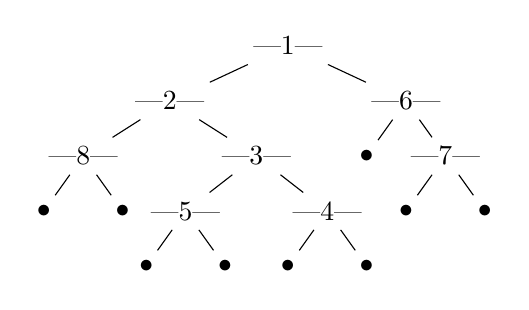
\begin{tikzpicture}[level 1/.style={sibling distance=3cm}, level
    2/.style={sibling distance=2.2cm}, level 3/.style={sibling
      distance=1.8cm}, level 4/.style={sibling distance=1cm}, level
    distance = 7mm]
    \node{\lstinline|1|} child { node {\lstinline|2|} child [level
      3/.append style={sibling distance=1cm}]{ node {\lstinline|8|}
        child { node {\leaf}} child { node {\leaf}}} child { node
        {\lstinline|3|} child { node {\lstinline|5|} child { node
            {\leaf}} child { node {\leaf}}} child { node
          {\lstinline|4|} child { node {\leaf}} child { node {\leaf}}
        }}} child[level 2/.append style={sibling distance=1cm}] { node
      {\lstinline|6|} child { node {\leaf}} child[level 3/.append
      style={sibling distance=1cm}] { node {\lstinline|7|} child {
          node {\leaf}} child { node {\leaf}}}} ;
  \end{tikzpicture}
  \hspace*{2em}
  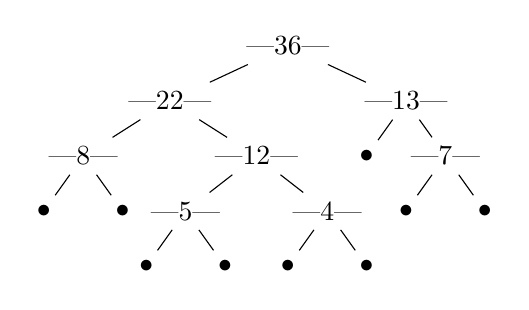
\begin{tikzpicture}[level 1/.style={sibling distance=3cm}, level
    2/.style={sibling distance=2.2cm}, level 3/.style={sibling
      distance=1.8cm}, level 4/.style={sibling distance=1cm}, level
    distance = 7mm]
    \node{\lstinline|36|} child { node {\lstinline|22|} child [level
      3/.append style={sibling distance=1cm}]{ node {\lstinline|8|}
        child { node {\leaf}} child { node {\leaf}}} child { node
        {\lstinline|12|} child { node {\lstinline|5|} child { node
            {\leaf}} child { node {\leaf}}} child { node
          {\lstinline|4|} child { node {\leaf}} child { node {\leaf}}
        }}} child[level 2/.append style={sibling distance=1cm}] { node
      {\lstinline|13|} child { node {\leaf}} child[level 3/.append
      style={sibling distance=1cm}] { node {\lstinline|7|} child {
          node {\leaf}} child { node {\leaf}}}} ;
  \end{tikzpicture}
\end{center}

% \caption{Tree transformation from \lstinline|aTree| (on the left) into tree \lstinline|t| (on the right)}
% \label{fig:trees}
% \end{figure}

%%% Local Variables:
%%% mode: latex
%%% TeX-master: "main"
%%% End:
